% Background:
%   Data parallelism and GPU computing.
%   Embedded languages
%

\chapter{Basics}
\label{ch:basics}

\epigraph{You see a wile, you thwart. Am I right?}%
{\textsc{---terry pratchett and neil gaiman}\\\textit{Good Omens}}

% TODO: introduction paragraph?

% This chapter introduces some basic ideas necessary to understand the design and
% implementation of Accelerate, our parallel array programming language. This
% chapter introduces parallelism and programming graphics processors for general
% purpose applications, before introducing the Accelerate language.


\section{Data parallelism}
\label{sec:data_parallelism}

The major processor manufacturers and architectures have long since run out of
room with most of the traditional approaches to boosting CPU performance.
Instead of driving clock speed and straight-line instruction throughput,
the inclusion of multiple cores on a single chip has become the dominant
mechanism for scaling processor performance. Despite this trend being apparent
for a number of years, programming parallel computers still remains an extremely
challenging task --- even for expert computer programmers, let alone for
scientists in other disciplines.

One programming model that has shown to make good use of parallel hardware is
\indexe{data parallelism}.
% The idea is that the application of an operation over
% a collection of data, such as an array, can often be performed in parallel.
Data parallelism focuses on distributing the data over the available processors,
and for each processor to perform the \emph{same} task on the \emph{different}
pieces of distributed data. To the programmer, data parallelism exposes a single
logical thread of execution that is fairly easy to understand and reason about.
In addition to its simplicity, the data parallel approach to programming
parallel computers has several advantages:
%
\begin{enumerate}
\item The model is independent of the number of processors, so it scales to any
    number of processors by decomposing data into the appropriate number of
    chunks.

\item All synchronisation is implicit, so the programming model is safe from
    race conditions, eliminating a major source of errors in parallel programs.

\item As memory bandwidth is often a limiting factor in modern computers, the
    emphasis on data layout can assist with both data flow as well as
    parallelisation.
\end{enumerate}
%
In the world of massively parallel computing with strong locality requirements,
data parallelism is the well established, demonstrably successful brand leader.
Examples of data parallel programming environments include High Performance
Fortran (HPF)~\cite{HPF:1997}, the collective operations of the Message Passing
Interface (MPI)~\cite{MPI:2012}, Google's Map/Reduce
framework~\cite{Dean:2008fi}, and NVIDIA's CUDA\cuda{} API for graphics
processors~\cite{NVIDIA:2012wf}.


\section{GPU computing} % {GPGPU programming is data parallel programming}
\label{sec:gpu_computing}

\cuda[|(]{}
\gpu[|(]{}

General-purpose computing on graphics processing units (GPGPU\gpgpu)
is the utilisation of a graphics processing unit (GPU\gpu) ---
which typically handles the computations for computer graphics --- to perform
computations in applications typically handled by the central processing unit
(CPU). Since general purpose CPUs are designed to optimise the performance of a
single thread of execution, much of the processor's resources (die area and
power) are dedicated to non-computational tasks such as caching and branch
prediction. Conversely, the highly parallel nature of graphics processing
(\indext{rasterisation}) means the GPU architecture can instead use these
resources to execute many tasks in parallel, improving the computational
throughput for parallel workloads at the expense of decreased single threaded
performance. This difference in architectures between the CPU and GPU is
illustrated in Figure~\ref{fig:cpu_gpu_block_diagram}.

\begin{figure}[tbp]
    \centering
    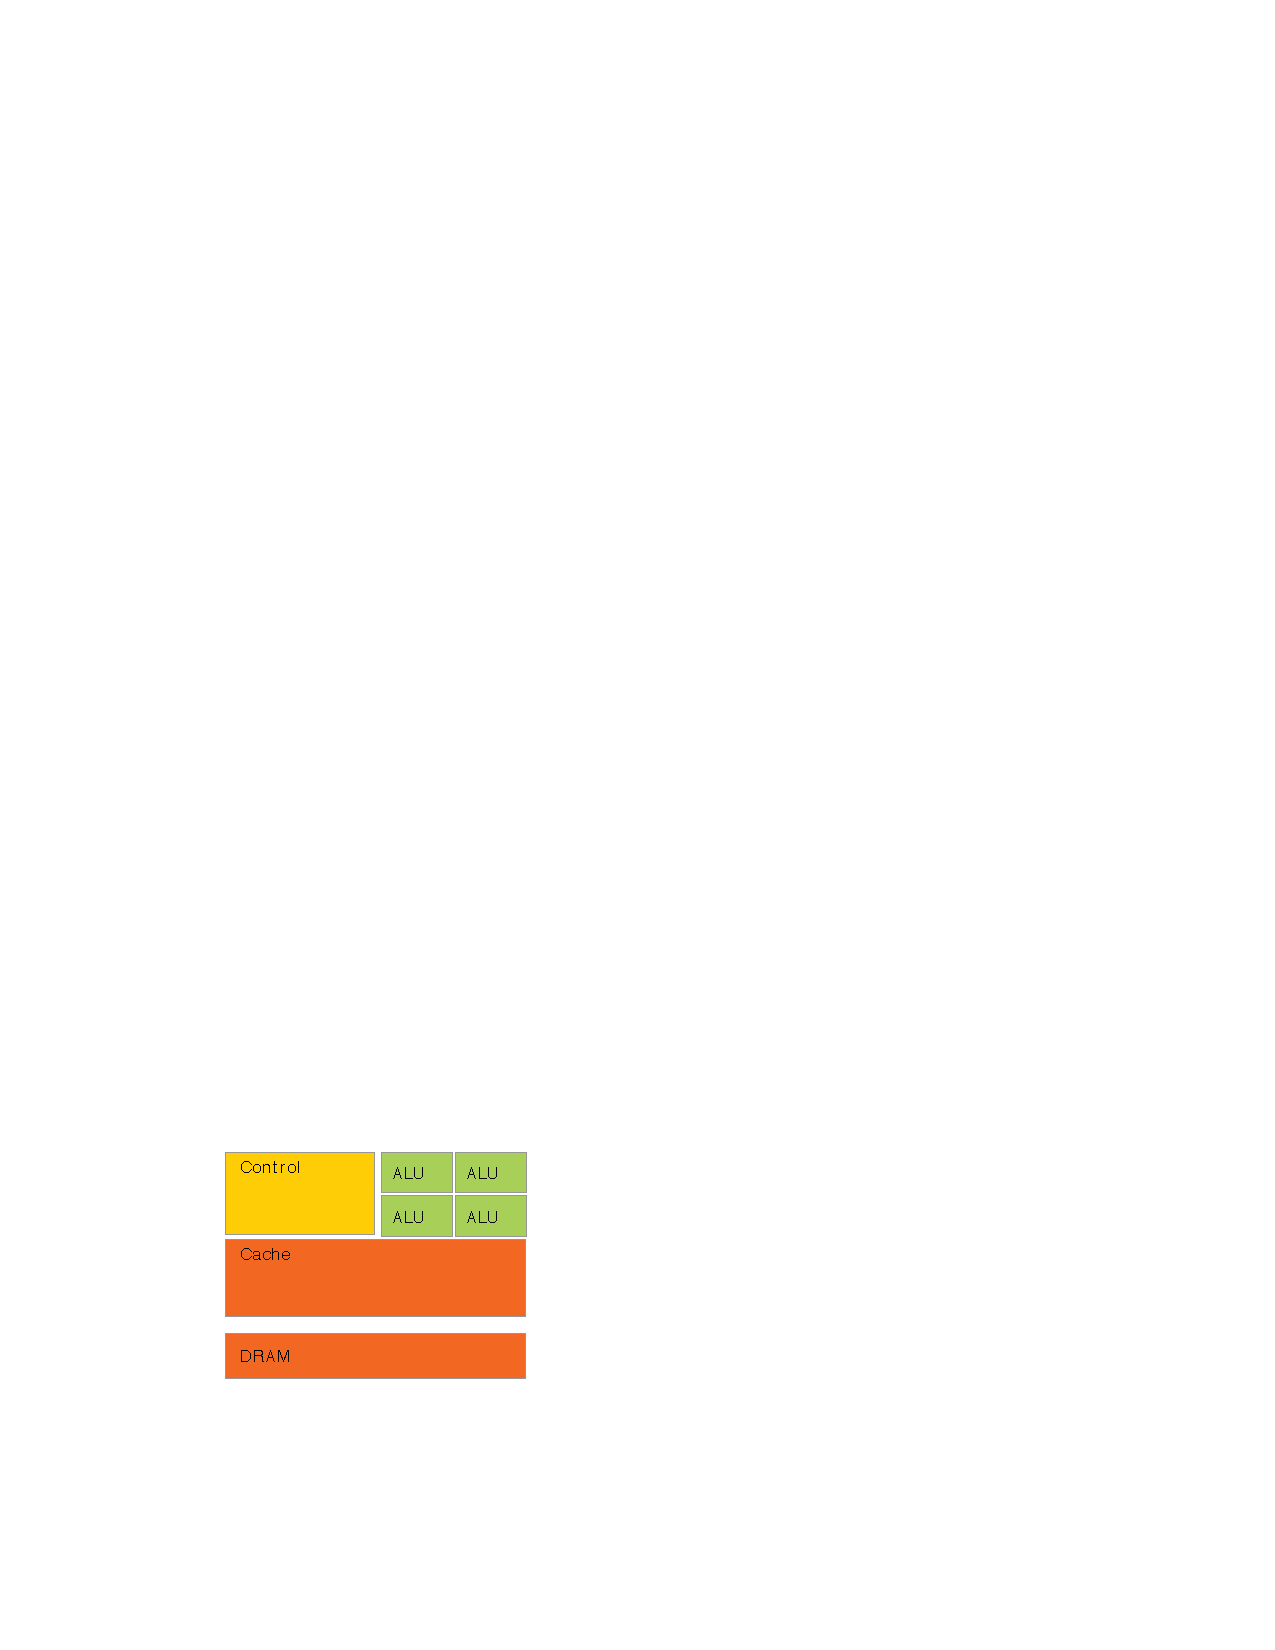
\includegraphics[width=0.4\textwidth]{images/basics/block_cpu}
    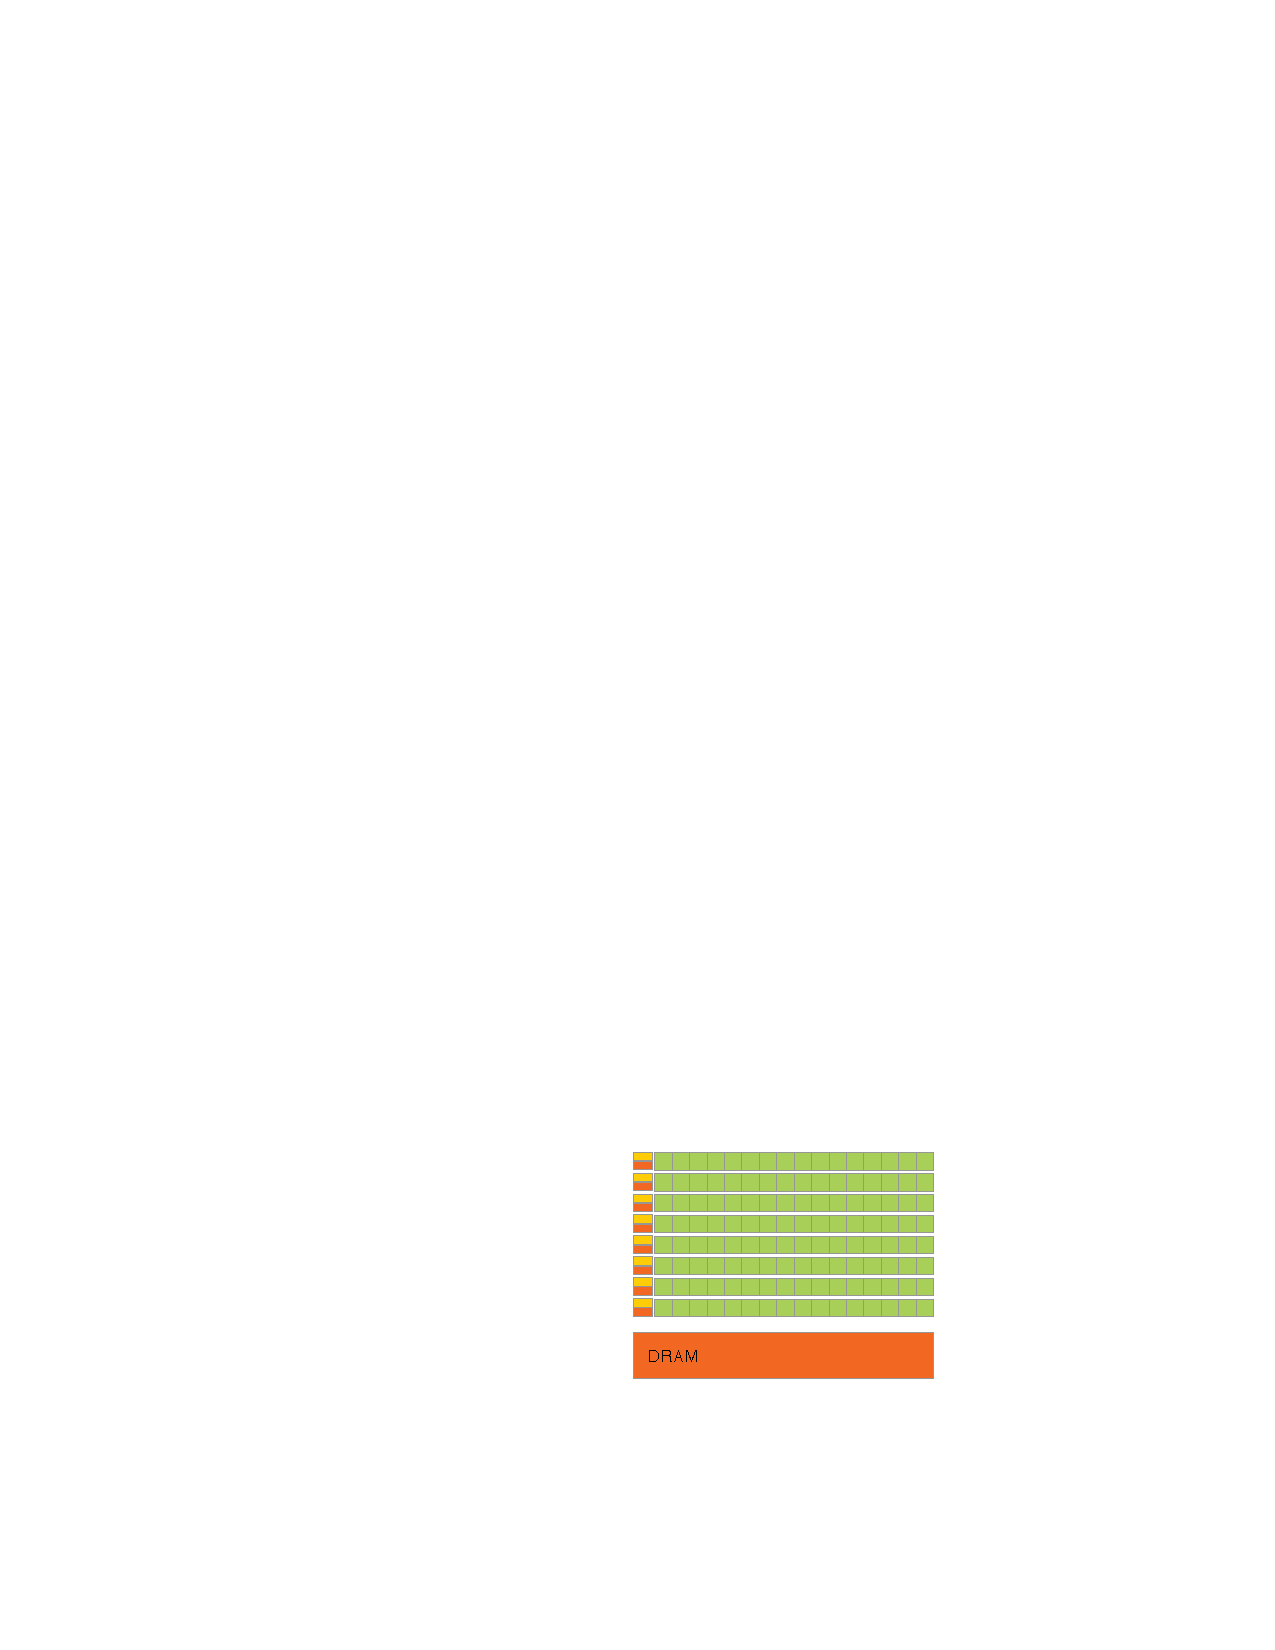
\includegraphics[width=0.4\textwidth]{images/basics/block_gpu}
    \caption[Block diagram comparing CPU and GPU architectures]{Block diagram
    comparing the relative use of transistors in a CPU (left) compared to a GPU
    (right). The GPU is specialised for highly parallel, compute intensive
    workloads, and so is designed such that the majority of its transistors are
    devoted to data processing, rather than data caching and control flow.
    Images from~\cite{NVIDIA:2012wf}.}
    \label{fig:cpu_gpu_block_diagram}
\end{figure}

More specifically, the GPU\gpu{} is especially well suited to executing
problems that can be expressed as data parallel computations, where the same
program is executed by many processors on many different data elements in
parallel (\S\ref{sec:data_parallelism}). Because the same program is executed by
many processors, there is no need for sophisticated control flow, and because it
is executed on many data elements, memory access latency can be hidden with
calculations rather than by big caches. Many applications that process large
data sets can use the data parallel programming model to speed up calculations,
and these applications can often be coded to execute on the GPU\@.


\section{CUDA}
\label{sec:cuda}

The CUDA\cuda{} architecture is the parallel computing platform and
programming model created by NVIDIA and implemented by the graphics processing
units (GPUs\gpu) that they produce. Using CUDA, programmers gain direct access
to the memory and massively parallel multicore architecture of the GPU, which
can then be used for general purpose computing applications, not just graphics.

CUDA\cuda{} extends the C programming language by allowing the programmer to define
functions, called \emph{kernels}\cuda[kernel]{}, that, when called, are
executed $n$ times in $n$ data parallel threads on the available processing
elements, rather than only once like regular C functions. These functions are
executed by threads in SIMD groups called \emph{warps}\cuda[warp]{} arranged in
a multidimensional structure of \emph{thread blocks}\cuda[thread block]{}.
Within a warp, all threads execute the same instructions in lock-step, so
divergent control flow must be handled via predicated execution.
Threads within a block can cooperate by sharing data through some \emph{shared
memory}\cuda[shared memory]{} and by synchronising their execution to coordinate
memory access. More precisely, the programmer can specify synchronisation points
in the kernel by calling @__syncthreads()@\cuda[\code{__syncthreads()}]{}, which
acts as a barrier at which all threads in the block must wait before any are
allowed to proceed. Each thread block executes independently of each other, so a
GPU with a higher number of CUDA cores --- or \emph{streaming
multiprocessors}\cuda[streaming multiprocessor]{} (SM) --- will execute the
program in less time than a GPU with fewer multiprocessors.

\begin{lstlisting}[style=cuda_float
    ,label=lst:cuda_vecadd
    ,caption={[CUDA kernel for pair wise addition of two vectors]A CUDA kernel
        that illustrates pair wise addition of two vectors. The
        \code{__global__}\cuda[\code{__global__}]{} keyword marks a function as
        a kernel that should be executed on the GPU in data parallel. The
        execution configuration syntax \code{<<<...>>>} specifies the number of
        threads that will each execute the function in data parallel.}]
// Kernel definition
__global__ void VecAdd(float *A, float *B, float *C, int N)
{
    int i = blockIdx.x * blockDim.x + threadIdx.x;

    if (i < N) {
        C[i]  = A[i] + B[i];
    }
}

int main()
{
    ...
    // Kernel invocation with N threads
    int threadsPerBlock = 128;
    int numBlocks       = (N + threadsPerBlock - 1) / threadsPerBlock;
    VecAdd<<<numBlocks, threadsPerBlock>>>(A, B, C, N);
    ...
}
\end{lstlisting}

As an example, Listing~\ref{lst:cuda_vecadd} illustrates the pair wise addition
of two vectors $A$ and $B$ of size $N$ each, and stores the result in a vector
$C$. The kernel is defined with the @__global__@\cuda[\code{__global__}]{}
declaration specifier. The number of CUDA\cuda{} thread blocks and the number of
threads in each block that execute the kernel, at this invocation, is specified
in the @<<<...>>>@ syntax. Moreover, Listing~\ref{lst:cuda_vecadd} demonstrates
that the GPU\gpu{} programming model as exposed by CUDA is a data parallel
programming model --- $N$ threads execute $N$ individual instances of the kernel
function @VecAdd@, and each thread operates on a single element of each input
array to create a single value in the result. See the CUDA\cuda{} C programming
guide for details~\cite{NVIDIA:2012wf}.


\section{Data parallel algorithms in CUDA}
\label{sec:parallel_algorithms_in_cuda}

CUDA\cuda{} is a parallel computing platform for programming NVIDIA GPUs.
Using CUDA, the GPU\gpu{} becomes accessible not just for graphics applications,
but for computational tasks much like a CPU\@. Unlike CPUs, however, GPUs have a
parallel throughput architecture that emphasises executing many concurrent
threads slowly, rather than executing a single thread very quickly.
% Unlike CPU cores, instructions are issued in order and there is no
% branch prediction and no speculative execution.
See Section~\ref{sec:cuda} for more information.

% The CUDA hardware architecture is built around a scalable array of
% multithreaded \emph{streaming multiprocessors} (SMs).\index{SM|see {streaming
% multiprocessor}}\index{streaming multiprocessor} When a CUDA program on the
% host CPU invokes a \indexe{kernel} --- a function which executes on the GPU
% --- a \emph{grid} of threads grouped into equally sized \emph{blocks} is
% % \index{thread!grid} \index{thread!block}
% enumerated and distributed to the multiprocessors for execution, using a
% \emph{single-instruction, multiple thread} (SIMT) model.\index{SIMT|see {single
% instruction multiple thread}}\index{single instruction multiple thread} The
% multiprocessor creates, manages, schedules, and executes threads in groups of 32
% parallel threads call a \indexe{warp}. All threads in a warp share a single
% program address counter, so divergent threads within a warp are handled via
% predicated execution; for example the positive and negative cases of a branch
% are executed in sequence, with threads not on the current execution path made
% inactive (disabled). In essence, streaming multiprocessors replace the complex
% instruction scheduling logic of a CPU which increases single threaded
% performance --- namely out-of-order execution, branch prediction and speculative
% execution --- with many additional ALUs (arithmetic logic units, often referred
% to as CUDA cores) all executing the same instruction sequence in parallel in
% order to increase total instruction throughput. Details of the CUDA
% architecture can be found in the CUDA C programming
% guide~\cite{NVIDIA:2012wf}; we present only those features required for the
% discussion.

Some collective operations such as @map@ have an obvious mapping to the
highly parallel CUDA architecture, so we elide discussion of their
implementation. Other collective operations such as @scan@, where the value
of each element depends on the value of the previous last, may at first seem to
not admit a parallel interpretation at all. This section outlines the
implementation of this second kind of collective operation, where efficient
parallel implementation in CUDA may not be obvious.


\subsection{Reduction}
\label{sec:parallel_reduction}

Reductions are a common and important data-parallel
primitive~\cite{Chatterjee:2009vh}. Figure~\ref{fig:tree_reduction} illustrates
the basic strategy for reducing an array in parallel. Within each thread block a
tree-based approach is used to reduce elements to a single value, and multiple
thread blocks each process a portion of the array in parallel. However, there is
no global synchronisation primitive in CUDA that can be used to combine the
partial results. This is because global synchronisation would be (a) expensive
to build in hardware for large numbers of multiprocessors, and (b) difficult for
programmers to use without introducing sources of deadlock. Instead, kernel
launches serve as a global synchronisation point, so thread blocks instead
communicate their partial results by committing them to memory, and the kernel
is launched recursively until the final reduction value is computed.

\begin{figure}
    \begin{center}
        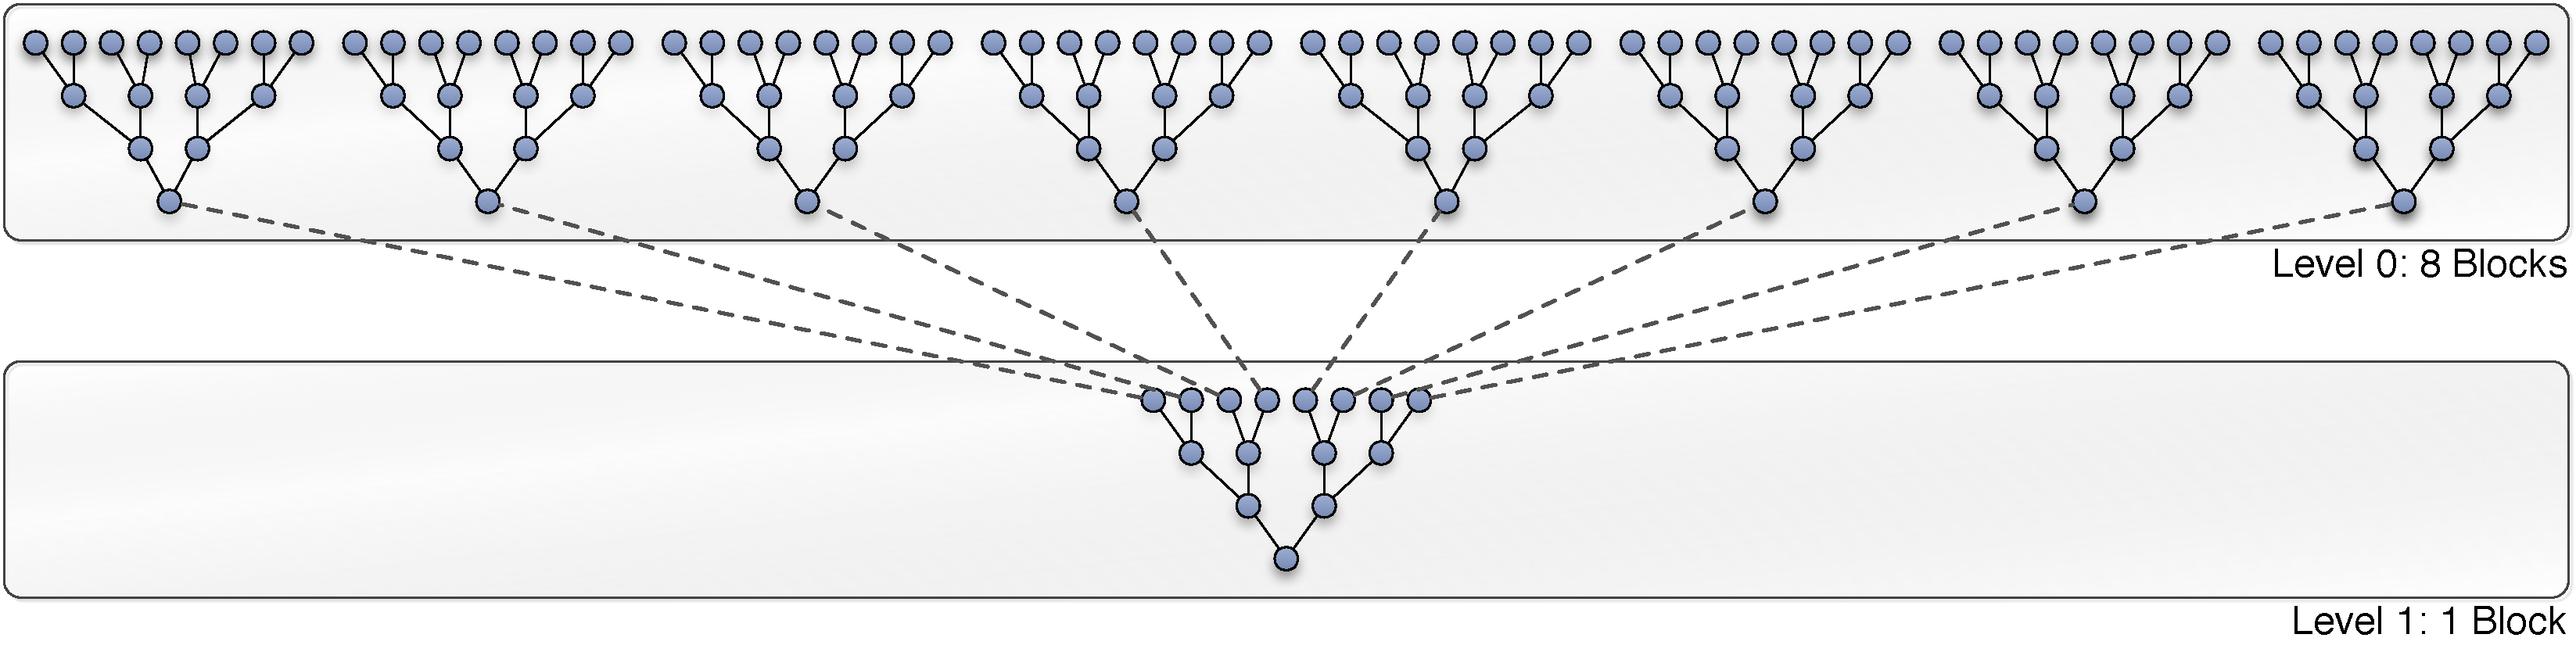
\includegraphics[width=\textwidth]{images/basics/tree-reduction}
    \end{center}
    \caption[A parallel tree reduction]{Illustration of a tree reduction,
        performed in two steps. In the first step 8 thread blocks in parallel
        reduce eight segments of the array to a single element each. The thread
        blocks synchronise by writing their result to memory, and the kernel is
        called recursively until the final scalar result is computed.}
    \label{fig:tree_reduction}
\end{figure}

Note that if we wish to fuse\fusion{} other operations into the fold kernel,
only the first line of reductions at level zero perform the fused operation. All
subsequent reductions in that kernel, as well as the recursive steps at level
one and beyond, are pure reductions. We discuss fusion further in
Section~\ref{sec:array_fusion}.
% Thus, the fused operation requires compilation of two separate kernels.
% We focus on the level zero kernel, which is more interesting.

\subsubsection{Parallel Reduction Complexity}
\label{sec:parallel_reduction_complexity}

% \marginnote{tk: for non power-of-2 n, add upper/lower bounds symbols}
If each thread combines two elements at a time, then a vector of length $N$ will
be reduced in $\mathcal{O}\left( \log N \right)$ parallel steps. Each step $S$
does $\sfrac{N}{2^S}$ independent operations, so the \emph{step
complexity}\index{complexity!step} of the algorithm is:
\[
\mathcal{O}\left( \log N \right)
\]
For $N=2^{D}$, the algorithm thus performs $\sum_{S=1}^{D}2^{D-S} = N - 1$
operations. This means that the \emph{work complexity}\index{complexity!work} of
the algorithm is:
\[
\mathcal{O}\left( N \right)
\]
and therefore does not perform more work than a sequential algorithm. For $P$
threads running physically in parallel on $P$ processors, the \emph{time
complexity}\index{complexity!time} is $\mathcal{O}\left( \sfrac{N}{P} + \log N
\right)$. In a thread block $N = P$, so the time complexity is:
\[
\mathcal{O}\left( \log N \right)
\]
Compare this to a sequential reduction, which has a time complexity of
$\mathcal{O}\left( N \right)$.

\subsubsection{Algorithm Cascading}
\label{sec:algorithm_cascading}

The \emph{cost} of a parallel algorithm is the number of processors $\times$
time complexity. This implies that the cost of the algorithm is
$\mathcal{O}\left( N \log N \right)$, which is \emph{not} cost efficient.

Brent's theorem~\cite{Chatterjee:2009vh} suggests that instead of each thread
summing two elements, \emph{algorithm cascading} can be used to combine a
sequential and parallel reduction. If each thread does $\mathcal{O}\left( \log N
\right)$ sequential work, this will reduce the cost of the algorithm to
$\mathcal{O}\left( \sfrac{N}{\log N} \log N \right)$, or rather:
\[
\mathcal{O}\left( N \right)
\]
while keeping the work complexity $\mathcal{O}\left( N \right)$ and step
complexity $\mathcal{O}\left( \log N \right)$.

As an example, this result implies that each block of 256 threads should sum a
total of $256 \times \log_2 \left( 256 \right) = 2048$ elements. In practice it
is beneficial to do even more sequential work per thread, as this will reduce
the number of levels in the recursive tree reduction, and provide better latency
hiding by minimising the number of thread blocks launched.


\subsubsection{Mapping to CUDA Threads}

Reduction of a one dimensional array uses multiple thread blocks\cuda[thread
block]{} to cooperatively reduce the array, as described above. The number of
thread blocks used is limited to the maximum number which can be simultaneously
resident on the current device. This may require each thread to do more
sequential work than that indicated by the algorithm cascading analysis,
but limits the total kernel startup cost associated with launching thread
blocks. Since the maximum number of resident thread blocks is typically much
less than the number of threads in a block, the reduction will require at most
two kernel invocations.\footnote{Accelerate selects the thread block size in
order to maximise thread occupancy. As this depends on both the specific GPU
being used as well as the user function the array is reduced with, an upper
bound of two parallel steps can not be guaranteed. See
Section~\ref{sec:launch_configuration} for more information.}

Higher-dimensional reductions reduce the array along the innermost dimension
only.
% This is similar to a segmented fold, except that the segment descriptor is
% not necessary since the length of every segment is the same and can be
% determined directly from the extent of the input array.
Instead of all thread blocks
cooperatively reducing each segment sequentially, each segment is reduced by a
single thread block which operates independently of all other thread blocks. A
consequence of this is that proper device utilisation depends on the shape of
the array and not simply the total number of elements in the array. For example,
reduction of an array stored as a $1 \times n$ matrix will use one thread
block to reduce the single matrix row,
no matter how large $n$ is. This simplifies the implementation but is clearly
not always ideal.\footnote{The number of multiprocessors on a device various
between architecture generation and performance of a given card. For example, a
Tesla T10 processor (compute capability 1.3) has 240 cores split over 30
multiprocessors, while a Kepler K20X processor (compute capability 3.5) has 2688
cores split over only 14 multiprocessors. A given architecture generation will
have the same number of cores per multiprocessor, and lower performance
processors in a generation are produced by incorporating (or activating) fewer
multiprocessors, thereby reducing the total core count.}


\subsection{Scan}
\label{sec:parallel_scan}

Parallel scan and segmented scan algorithms are a crucial building block for a
great many data-parallel algorithms~\cite{Blelloch:1990ts,Chatterjee:1990vj}.
They also form the basis for efficiently mapping nested data-parallel languages
such as NESL~\cite{Blelloch:1995ut,Blelloch:1996jx} on to flat data-parallel
machines. Because of their fundamental importance to many algorithms,
implementing efficient scan operations in CUDA\cuda{} has received much
attention~\cite{Sengupta:2007tc,Sengupta:2008ut,Dotsenko:2008fo,Merrill:2009un,Harris:2012fy}.

\begin{figure}
    \begin{center}
        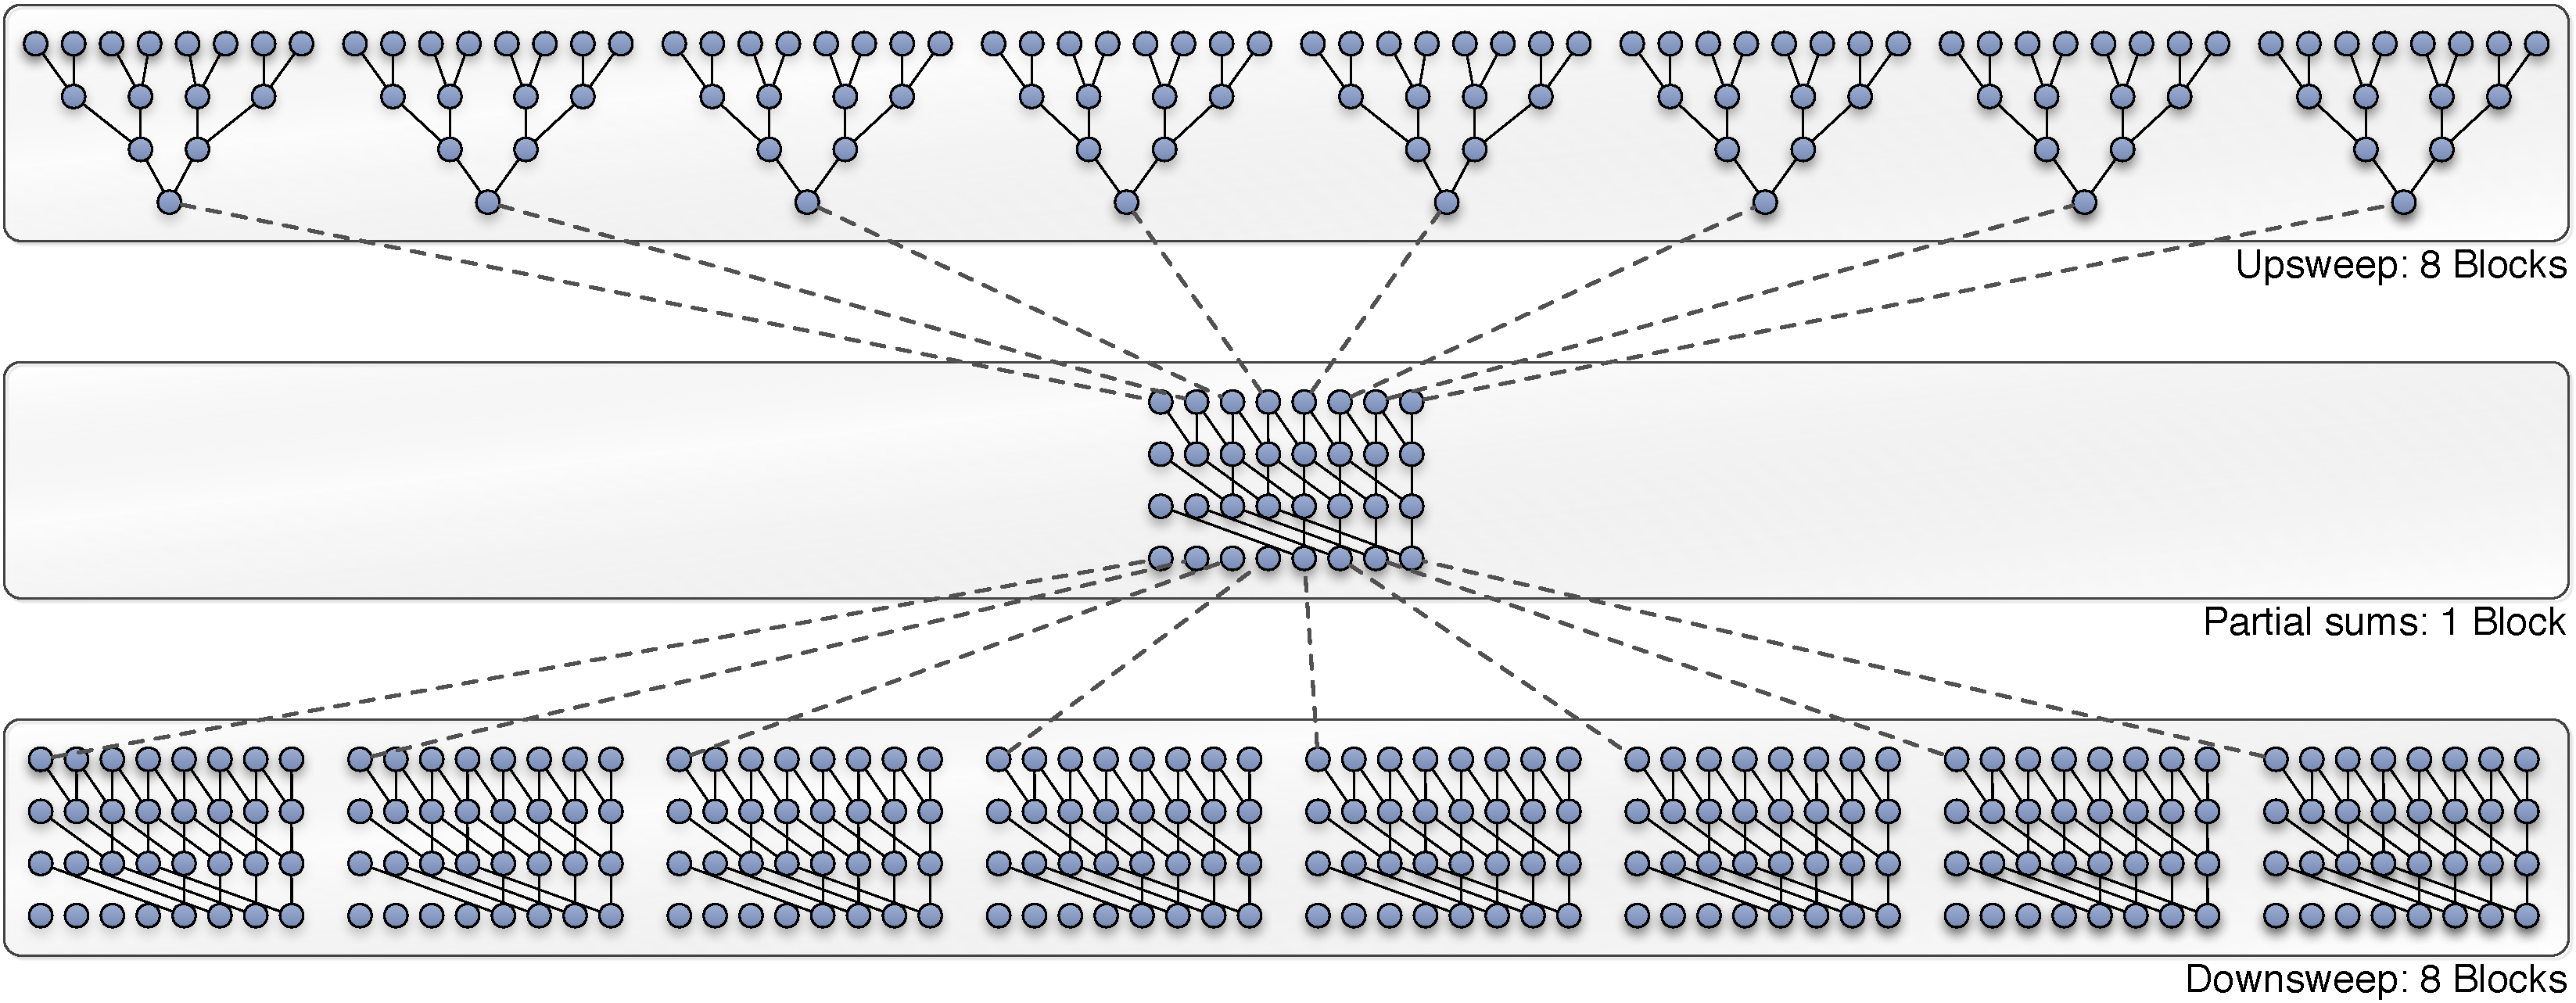
\includegraphics[width=\textwidth]{images/basics/scan}
    \end{center}
    \caption[A parallel inclusive scan]{Illustration of a parallel inclusive
        left-to-right scan, which is performed in three steps. In the first
        step, 8 thread blocks compute the partial scan result for each eight
        element section of the array. The partial results are then scanned by a
        single thread block in the second step. In the final phase, the 8 thread
        blocks use the partial results as the initial element when computing the
        final scan result for this section of the array.}
    \label{fig:fast_scan}
\end{figure}

The basic binary-tree based scan algorithm proceeds in $\log
N$\index{complexity!step} stages.
% As shown in Figure~\ref{fig:fast_scan}, the binary operator is applied to two
% distinct elements of the input array and the output is stored into a new array.
In order to compute scans efficiently on the GPU\gpu{}, the input array is
decomposed into a number of blocks of size $B$, such that an inclusive scan of
$B$ elements can be computed by an individual thread block\cuda[thread block]{},
locally in shared memory\cuda[shared memory]{}\cuda{}. The inclusive scan
algorithm depicted in Figure~\ref{fig:fast_scan} proceeds in three phases:
%
\begin{enumerate}
\item The input array is divided into chunks of size $B$ elements and
    distributed to the thread blocks\cuda[thread block]{}, which each scan their
    portion of the array in parallel. The final scan value (partial result) from
    each thread block @i@ is stored into an intermediate array
    @block_results[i]@. Note that even though we require only the final value,
    since scans are directional --- either to the left or right --- we must
    compute the entire scan and return only the last value, to ensure that
    elements are processed in the correct left-to-right or right-to-left order.

\item A single thread block performs a scan of the helper array @block_results@.
    Accelerate is set up such that the number of blocks in the first step is
    less than the maximum thread block size (\S\ref{sec:executing_programs}), so
    this step does not need to repeatedly apply the global scan algorithm.

\item All blocks scan their section of the input array in parallel again, where
    thread block @i@ uses element @i@ of the result of step 2 as the initial
    element of the scan.

\end{enumerate}

For an exclusive scan, it is also necessary to ensure that the computation of
the partial block sums includes the seed element.


\subsubsection{Inclusive vs. Exclusive scan}

The above description mentions two different flavours of scans. The output of an
exclusive scan at each location is a function of all the elements that came
before it, but does \emph{not} include the current element. On the other hand,
the inclusive scan is a function of all elements up to and \emph{including} the
current element. At an example, the two methods produce the following output for
a left-to-right prefix sum:
%
\begin{lstlisting}[style=haskell]
  input          = [ 13,  7, 16, 21,  8, 20, 13,  12 ]
  exclusive scan = [  0, 13, 20, 36, 57, 65, 85,  98 ]
  inclusive scan = [ 13, 20, 36, 57, 65, 85, 98, 110 ]
\end{lstlisting}

These methods are well known in data-parallel programming, and some algorithms
are best expressed in terms of one or the other.
% Accelerate supports both of these styles of scan
% In Accelerate, we follow the behaviour of the standard Haskell @scan@ family
% of functions. Namely, @scan*1@ is an inclusive scan, while @scan*@ is an
% exclusive scan but also includes the final element, thus increasing the size
% of the output array by one.


\subsubsection{Interaction with array fusion}

In the scan algorithm described above, the input array to be scanned is read
twice: once when computing the partial block results, and a second time when
computing the final scanned array. If the input does not refer to manifest array
data, but instead an array in a symbolic form resulting from array
fusion\fusion{} (\S\ref{sec:array_fusion}), then the elements of the delayed
array --- which might contain arbitrarily expensive computations --- will be
computed twice also.

In order to avoid this, in some circumstances it might be beneficial for either
(a) the first phase of the scan to store the entire partial scan result, rather
than just the final element; or (b) to always read in manifest data, effectively
disallowing producer/consumer fusion\fusion{} (\S\ref{sec:array_fusion}) for
scans in the CUDA\cuda{} backend. The latter option is undesirable, and the
former may not work for non-commutative operators, such as the one we used in
the operator-transformation-based definition of segmented scan. Currently the
user has no control as to whether the input array is manifest or delayed, and no
special action is taken on the part of the backend in its current
implementation, although both alternatives are possible.

% It is left to future work to fully investigate this interaction between array
% fusion and operations such as scan, where the underlying implementation requires
% multiple passes over the input data.

% In order to avoid this, it might seem that one approach could be for each thread
% block in the first phase to write its entire partial scan result to memory,
% which would include any computations that were part of the fused array, rather
% than just the final element. In the third phase, each block would then combine
% the partial result from the second stage to each element of the partial scan
% result from the first phase (in effect a @map@ operation). However, this would
% not correctly handle non-commutative operators, something we took advantage of
% in the definition of segmented scans.


\subsection{Permute}
\label{sec:parallel_permute}

The @permute@ collective operation defines a forward permutation $f$ as an
index mapping from one array $X$ onto the result array $Y$, which we can write
as  $f : X \rightarrow Y$. Implementation of the permute function in Accelerate
is complicated because we have not placed any particular restrictions on $f$,
namely:
%
\begin{enumerate}
    \item $f$ is not \indext{surjective}: the range of $f$ may not cover the
        codomain $Y$. For every $x$ in $X$, $f\left( x \right)$ need not yield
        every index $y$ in $Y$. This means that the result array must first be
        initialised with a set of default values.

    \item $f$ is not \indext{injective}: distinct elements of the domain may map
        to the same element in the codomain. For all $x$ and $x'$ in $X$, if
        $f\left( x \right) = f\left( x' \right)$, we may have that $x \ne x'$.
        This means we require an associative combination function to combine
        elements from the domain that map to the same index in the codomain.

    \item $f$ is \indext{partial}: elements of the domain may be ignored, and
        thus do not map to elements in the codomain.
\end{enumerate}

That the permutation function admits partial functions in the index mapping is
not particularly challenging for the implementation, and indeed is useful for
implementing the @filter@ operation, shown in Listing~\ref{lst:filter}. The
special value @ignore@ is used to drop elements of the input vector that do not
satisfy the predicate, by not mapping those indices to an index in the codomain.
%
\begin{lstlisting}[style=haskell_float
    ,label=lst:filter
    ,caption={[Filtering a vector based on a predicate] Filtering returns only
    those elements of a vector which satisfy a predicate. This operation is
    included as part of Accelerate's standard prelude.}]
filter :: Elt a => (Exp a -> Exp Bool) -> Acc (Vector a) -> Acc (Vector a)
filter p vec
  = let flags            = map (boolToInt . p) vec
        (targetIdx, len) = scanl' (+) 0 flags
        defaults         = backpermute (index1 $ the len) id vec
    in
    permute const defaults (\ix -> flags!ix ==* 0 ? (ignore, index1 $ targetIdx!ix)) vec
\end{lstlisting}

On the other hand, because we can not prove that @filter@ is
\indext{surjective}, we require the result vector to be first initialised with
default values. Since we do not know anything about the element type @a@, the
only recourse is to copy elements from the input array @vec@. This is doubly
wasteful, because we must first execute the @backpermute@ kernel to compute the
@defaults@ array, and then copy those values into the results vector before
executing the @permute@ kernel, even though we know the initialised values
will be completely overwritten.

As a second example, Listing~\ref{lst:histogram} demonstrates the computation of
a simple ten bin histogram from a vector of floating point elements in the range
$\left[ 0, 100 \right)$. In this case the permutation function is neither
\indext{surjective} nor \indext{injective}, as some bins may contain no elements
and thus take the default value, while other bins may contain multiple elements
which need to be combined (accumulated) correctly.
%
\begin{lstlisting}[style=haskell_float
    ,label=lst:histogram
    ,caption={[A simple histogram] A simple histogram written in
    Accelerate. We assume the input vector contains elements in the range
    $\left[0,100\right)$ and accumulate into ten equally sized bins.}]
histogram :: Acc (Vector Float) -> Acc (Vector Int)
histogram vec
  = let bins      = 10
        zeros     = fill (constant (Z :. bins)) 0
        ones      = fill (shape vec)            1
    in
    permute (+) zeros (\ix -> index1 (A.floor ((vec ! ix) / P.fromIntegral bins))) ones
\end{lstlisting}

\subsubsection{Implementation using compare-and-swap}

The semantics of the @permute@ operation is that every permutation from source to result
array is applied at the same time in a single parallel step. If multiple
CUDA\cuda{} threads attempt a non-atomic write to the same memory location at
the same time, the writes will be serialised but the thread which performs the
final write is undefined, and so the final value at that memory slot is also
undefined~\cite{NVIDIA:2012wf}. To support non-injective permutation functions,
which are required to evaluate the histogram program correctly, the atomic
compare-and-swap operation is used to implement write combining.\footnote{The
atomic compare-and-swap operation on 32-bit values into global memory is only
available for devices of compute capability 1.1 and higher, and for 64-bit
values on devices of compute capability 1.2 and higher.} For a combination
function @f@ on elements of type @T@, the following atomically combines a value
from the source array @x@ with the value of the result array @y@:

\begin{lstlisting}[style=cuda]
  T x        = source[i];
  T y, old_y = result[j];
  do {
      y     = old_y;
      old_y = atomicCAS(&result[j], y, f x y);
  } while (y != old_y);
\end{lstlisting}
%
Any atomic operation on simple types can be implemented in terms of
compare-and-swap in this manner, although it would also be possible to use more
specific atomic operations such as @atomicAdd@\cuda{} in special cases.


\subsubsection{Implementation using explicit locking}

The implementation for combining elements of the permutation function works well
for simple atomic types, but as Accelerate uses a struct-of-arrays
representation (\S\ref{sec:representing_tuples}), combining tuple types must
apply the procedure to each component of the tuple separately. Because the
critical section does not apply to all components of the tuple at once, this can
lead to inconsistencies in the
result.\footnote{\url{https://github.com/AccelerateHS/accelerate/issues/137}}

One alternative for combining complex types is to explicitly lock each element
of the output array before threads can access it. Once a thread acquires the
lock on a particular element, it commits all components of the array as a single
atomic operation. A straightforward method to implement this is via a \emph{spin
lock}, where threads trying to acquire the lock simply wait in a loop
(``spin''), repeatedly checking whether the lock is available. Since the thread
remains active but is not performing any useful work, the use of this kind of
busy waiting is inefficient if threads are blocked for an extended period of
time --- for example, because the lock is contended by many threads, or the
atomic section executed while the lock is held is lengthy.

Implementing a standard spin-lock can be done as follows:
%
\begin{lstlisting}[style=cuda]
  do {
      old = atomicExch(&lock[i], 1);                                               // (1)
  } while (old == 1);                                                              // (2)
    /* atomic section */                                                           // (3)
  atomicExch(&lock[i], 0);                                                         // (4)
\end{lstlisting}
%
\begin{enumerate}
    \item The spin lock procedure requires a temporary array to represent the
        lock state for each element of the output array. We use 1 to represent
        the locked state, and 0 to indicate the element is unlocked. To lock
        element @i@ of the output array, we atomically store 1 into the @lock@
        slot for this element, returning the @old@ state of the lock.

    \item If the @old@ state of the lock was unlocked (0) then we have just
        acquired the lock. Otherwise, it was already locked, so we must retry.

    \item Once the lock is acquired, the atomic section can be computed.

    \item To release the lock, write zero back into the lock slot for this
        element. A memory barrier or atomic operation, as used here, is required
        for this step to ensure memory consistency on architectures which do not
        have a strong memory model, such as CUDA\cuda{} devices.
        % (later x86 architectures can safely use an unlocked @MOV@ instruction).

\end{enumerate}

% The current implementation does not use spin locking, but this is a possible
% alternative strategy for combining complex types in the permute operation.

However, a subtle problem emerges when we attempt to use the above algorithm. In
a CUDA device, all threads within a warp execute instructions in lockstep, and
divergent control flow is handled via predicated execution~(\S\ref{sec:cuda}).
Once a thread acquires a lock and exits the loop (2), it must wait for all other
threads in the warp to reach the same point, before execution of the critical
section (3) can begin. If two threads in a warp are attempting to acquire the
same lock, once the lock is acquired by one thread, that thread will sit idle
while the second thread spins attempting to grab a lock that will never be
released, because the first thread can not progress. The system is deadlocked.

In order to solve this problem, we must ensure that threads always make progress
once they have acquired the lock:
%
\begin{lstlisting}[style=cuda]
  done = 0;
  do {
      if (atomicExch(&lock[i], 1) == 0) {                                          // (2)
          /* atomic section */
          done = 1;
          atomicExch(&lock[i], 0);
      }
  } while (done == 0);                                                             // (1)
\end{lstlisting}
%
\begin{enumerate}
    \item The key change is that threads loop repeatedly until they have
        executed the entire critical section, rather than looping only to
        acquire the lock.

    \item If a thread fails to acquire the lock, it is disabled until the end of
        the branch. Threads that successfully acquire the lock enter the body of
        the conditional, where they execute the critical section and finally
        release the lock.
\end{enumerate}


\subsection{Stencil}
\label{sec:parallel_stencil}

Stencil operations are a fundamental building block of many scientific and image
processing algorithms. A stencil computation is similar to a @map@, that has
access to the elements in the local neighbourhood surrounding the element. For
example, at the core of many image processing algorithms is the
\indext{convolution} operator $*$, whose definition is as follows:

\begin{equation*}
    (A * K)(x, y) = \sum_i \sum_j A(x+i, y+j) K(i,j)
\end{equation*}
%
Here $A$ is the image being processed and $K$ is the \emph{convolution kernel}
or \indexe{stencil}. A \emph{stencil} is a small matrix that defines a
transformation on the image. Typical transformations include Gaussian blur and
the Sobel differentiation operator, both of which are used in the Canny edge
detection algorithm (\S\ref{sec:canny}).


\subsubsection{Bounds checking}

Since the stencil has access to elements in the surrounding neighbourhood, an
immediate concern is what to do when the stencil ``falls off'' the edge of the
array. Figure~\ref{fig:stencil3x3} shows the application of a $3\times3$
\indext{stencil} in this circumstance. The white squares indicate the
\emph{internal} region where the stencil is entirely within the array, and the
grey squares indicate the \emph{border} region, where part of the stencil lies
outside of the array boundary.

\begin{figure}[tbp]
    \begin{center}
        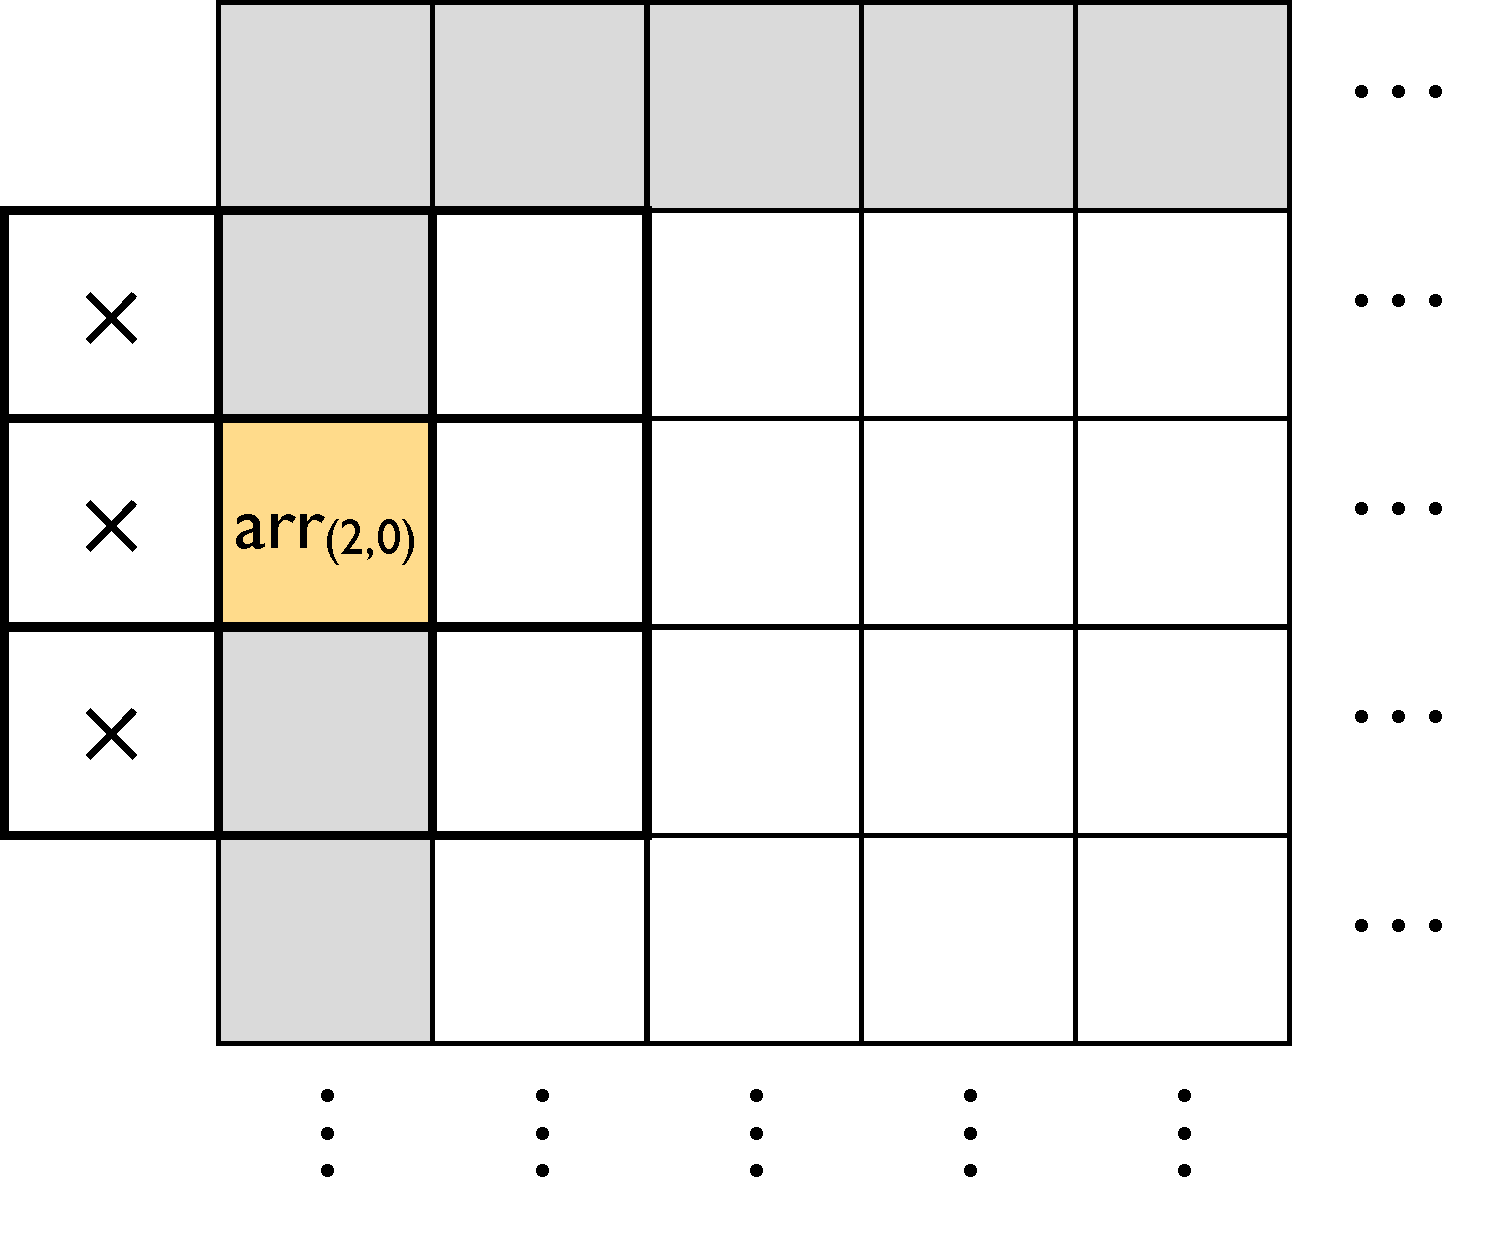
\includegraphics[width=0.5\textwidth]{images/basics/stencil3x3}
    \end{center}
    \caption[Application of a $3\times3$ stencil in the border region]
        {Application of a $3\times3$ stencil in the border region. If the focal
        point of the stencil, such as the indicated element at index
        \code{(Z:.2:.0)}, lies in the border region (grey), the neighbouring
        elements might fall outside the array bounds, whereas for elements in
        the internal region (white) the stencil lies entirely within the array.}
    \label{fig:stencil3x3}
\end{figure}

Boundary conditions determine how to handle out-of-bounds neighbours, by
specifying either a constant value to use instead, or by reading the source
array at a different index. However, with the array sizes typical of
GPU\gpu{} programs, the border region represents only a tiny fraction of the
entire array. For example, a 512-pixel square image has less than one percent of
its pixels along the edge. This fact implies that for optimal performance, we
should avoid testing of the boundary each time we read an element from the
source array. For simple convolutions\index{convolution} such as those used by
Canny (\S\ref{sec:canny}), this adds significant
overhead~\cite{Lippmeier:2011cd}.
%
The current implementation does not separate computation of the border and
internal regions.
% Separating computation of the border and internal region is left for future
% work.


\subsubsection{Overlapping elements}

Suppose we wish to apply a dense $3\times3$ \indext{stencil} to a single
internal point in the array, where every element of the stencil is utilised.
Application of the stencil requires at least nine elements of the array to be
loaded, and one store for the result.

\begin{figure}[tbp]
    \begin{center}
        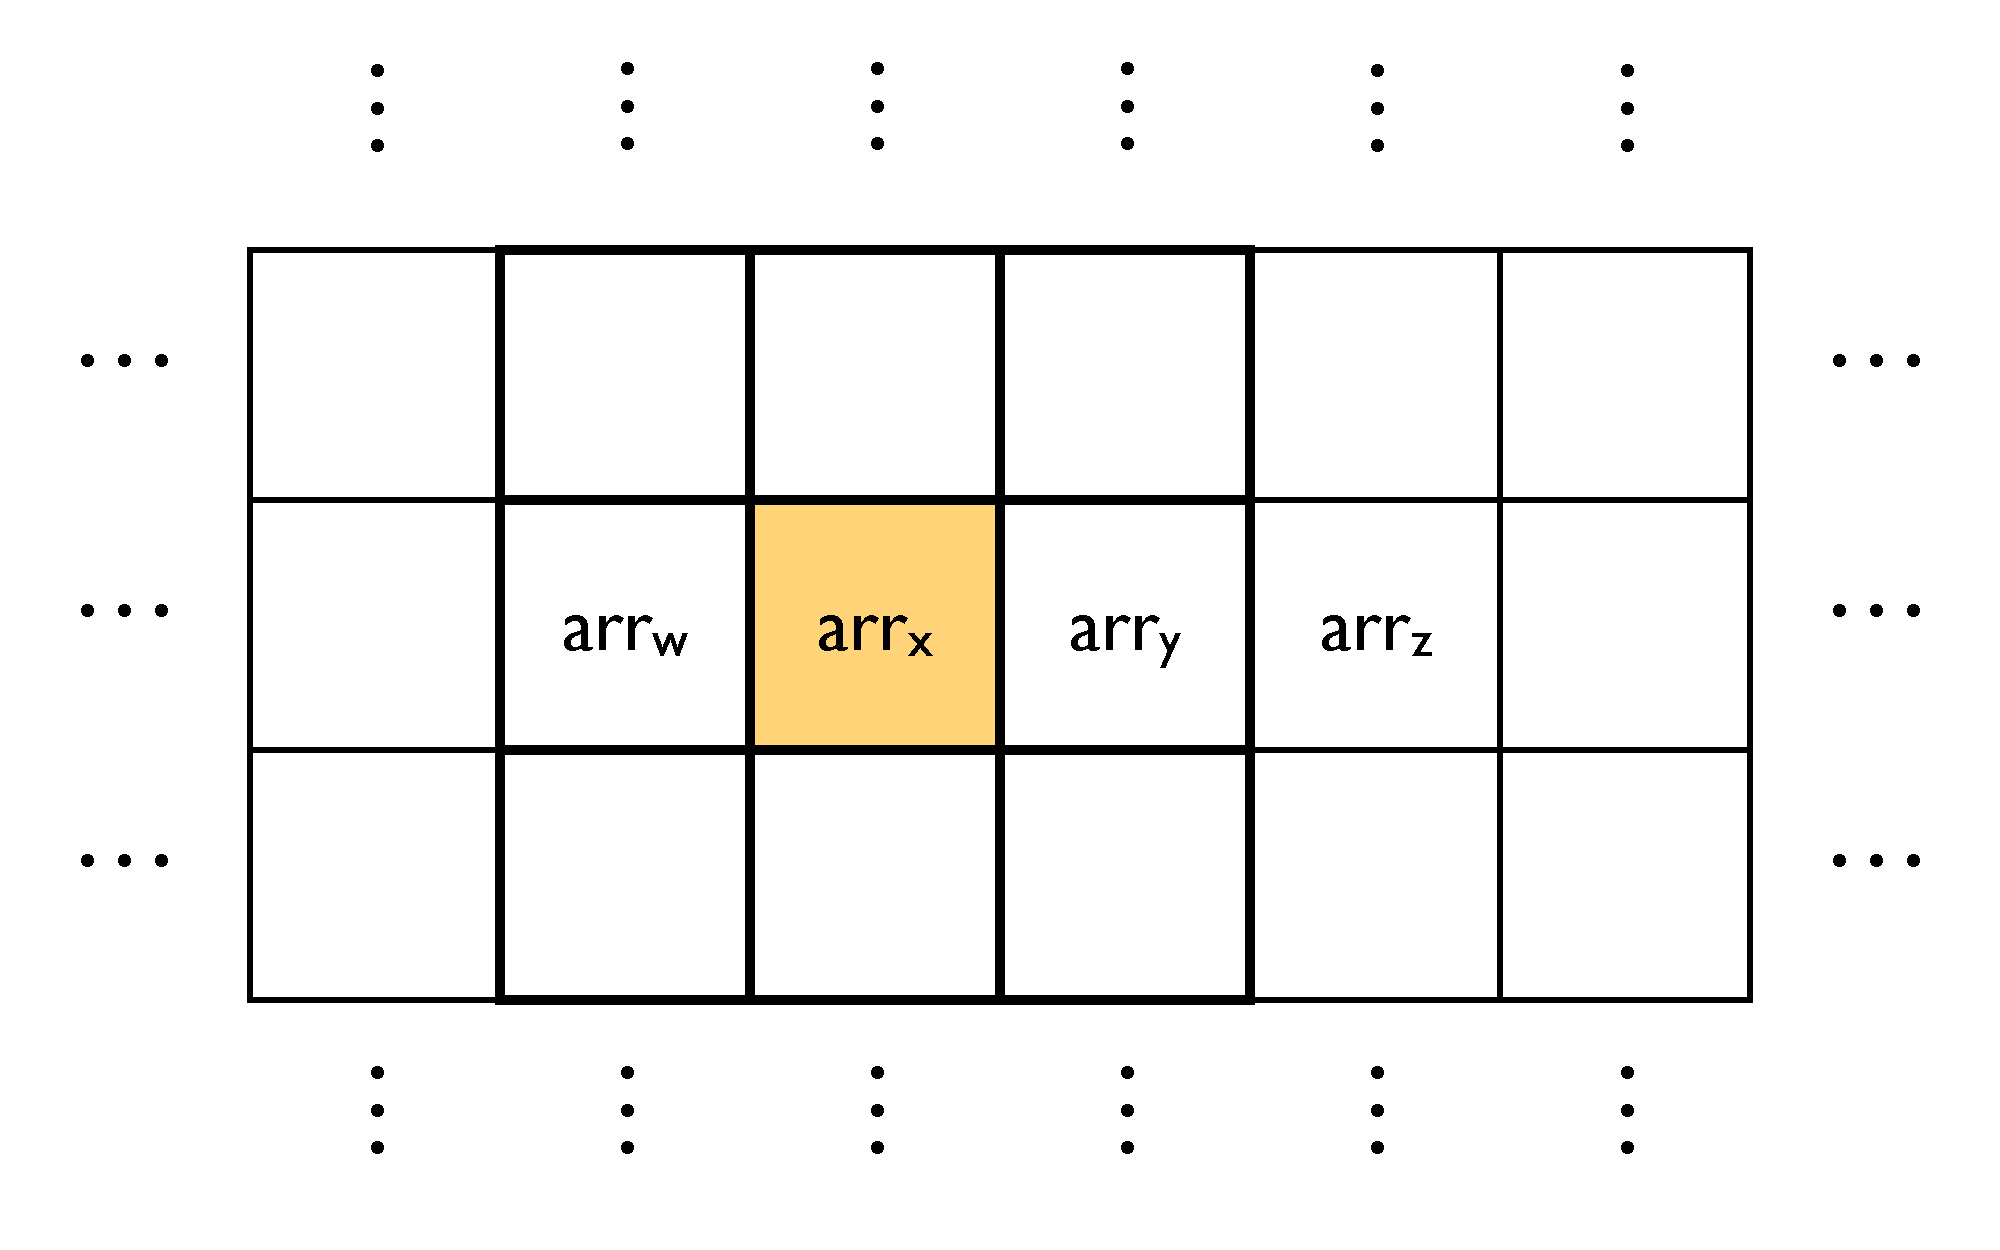
\includegraphics[width=0.6\textwidth]{images/basics/stencil-sharing}
    \end{center}
    \caption[Overlapping elements in a $3\times3$ stencil]{
        Overlapping elements in a dense $3\times3$ stencil. Computation of each
        element requires nine reads from the source array. If the four elements
        cooperate to share the source data, the number of loads to the source
        array is halved.}
    \label{fig:stencil_sharing}
\end{figure}

Figure~\ref{fig:stencil_sharing} shows the evaluation of four horizontally
adjacent elements. If we evaluate these points independently, we would need
$4 \times 9 = 36$ loads of the source array, plus the four stores to the result
array. However, if the calculation of these four elements can cooperate and
share loads from the source array into a local temporary array, this would
requires only $3 \times 6 = 18$ loads, plus the four stores. Sharing of stencil
elements can thus significantly reduce memory bandwidth requirements.

Sharing of stencil elements in CUDA\cuda{} can be achieved by having the thread
block\cuda[thread block]{} first cooperatively read the \indext{stencil}
elements into \cuda[shared memory]{} shared memory~\cite{NVIDIA:2012wf}, and
each thread then computes its stencil function using these shared values. In
Accelerate, sharing of stencil elements is complicated by two main factors:
%
\begin{enumerate}
    \item Stencil patterns can be large: up to 9 elements in each dimension.
        Since the shared memory region on the GPU is usually very small, this
        can significantly limit the maximum thread block size. If the occupancy
        of the device is too low, there may be insufficient parallelism to hide
        global memory transfer latency (\S\ref{sec:launch_configuration}).

    \item A stencil function does not need to use all elements defined in the
        pattern, so reading all elements into shared memory could waste more
        bandwidth than it saves. The pattern also does not need to be square nor
        symmetric, which complicates efficient cooperative loading of the
        common elements into shared memory.
\end{enumerate}

The implementation currently ignores this issue and does not explicitly share
elements between threads, and instead, relies on the hardware cache. For older
(compute 1.x) devices that lack a traditional cache mechanism to global memory,
we read the source array using the texture cache.\footnote{A holdover from the
graphical heritage of the GPU\gpu{}.} It is left to future work to investigate sharing
of stencil elements between threads, either in general or specialised for
certain cases such as dense stencils or those commonly used for
convolutions\index{convolution}.


\subsubsection{Interaction with array fusion}

Since the \indext{stencil} operation has access to the elements surrounding the
focal point of the stencil, if the input is represented by a symbolic array
resulting from array fusion\fusion{} (\S\ref{sec:array_fusion}), rather than
manifest array data, accessing these neighbouring elements implies recomputing
the symbolic computations on every element access. For some operation
@stencil s . map f@, if the results of @f@ can be shared between threads of the
stencil (previous section), or if @f@ is cheap, then the duplicate computations
required to fuse the two operations might be preferable to the extra memory
bandwidth required to store the result of @map f@ to memory. A full exploration
of stencil-aware array fusion is left to future work.


\subsection{Segmented operations}
\label{sec:segmented_operations}

The Accelerate language is restricted to programs which express only \emph{flat}
data parallelism. In this model, the computation executed in parallel on each
data element must itself be sequential. Although this model admits an efficient
implementation on highly parallel architectures and is ideally suited for
computations on dense, regular arrays, flat data parallelism is not as well
suited for algorithms that operate over \emph{irregular} structures, such as
sparse matrices, graphs, or trees.

On the other hand, \emph{nested data-parallel}
languages~\cite{Blelloch:1995ut,Levin:1994uu} allowing recursive data structures
and the application of parallel functions in data-parallel. The key insight is
that because the nested calls are to the same function, the \emph{flattening
transformation}~\cite{Blelloch:1988iu} can convert this nested data-parallelism
into an equivalent flat data-parallel program. An essential part of the
flattening transformation is the introduction of \emph{segmented} operations,
which apply a primitive operation in parallel to subcomponents of a nested
structure.

At an example, consider the following nested list of floating-point numbers:
%
\begin{lstlisting}[style=haskell]
  xss :: [ [ Float ] ]
  xss = [ [1,2], [3,4,5], [], [6] ]
\end{lstlisting}
%
The insight of the flattening transformation is to instead view this data
structure as a flat array of values, coupled with a \emph{segment descriptor}
encoding the length of each of the subsequences:
%
\begin{lstlisting}[style=haskell]
  xss' :: [ Float ]
  xss' = [ 1, 2, 3, 4, 5, 6 ]

  seg :: [ Int ]
  seg = [ 2, 3, 0, 1 ]
\end{lstlisting}
%
Operations on the nested data structure can then be transformed into segmented
operations over the flattened data:
%
\begin{lstlisting}[style=haskell,mathescape]
  map (fold f z xss) $\mapsto$ foldSeg f z xss' seg
\end{lstlisting}

Although we include support for several segmented operations in Accelerate, it
is left for significant future work to add support for the expression of nested
parallelism.


\subsubsection{Segmented reduction}

Segmented reduction is a primitive operations in Accelerate. Is is conceptually
similar to the multidimensional reduction, except that the length of each
segment is provided by the segment descriptor, rather than determined from the
extent of the input array.

In the current implementation, a segmented reduction uses a single
warp\cuda[warp]{} (SIMD group) to reduce each segment, although it would also be
possible to use the entire thread block, as is done for regular multidimensional
reductions. It remains to fully investigate which mapping is more efficient.


\subsubsection{Segmented scan}

Segmented scans are not implemented as primitive operations in Accelerate.
Instead, segmented scans are implemented in terms of unsegmented scans by
operator transformation~\cite{Schwartz:1980cy,Blelloch:1990ts}. Given the
operator $\oplus$ we can construct a new operator $\oplus^s$ that operators on a
flag-value pairs $\left( f_x, x \right)$ as follows:
%
\begin{equation*}
    \left( f_x, x \right) \oplus^s \left( f_y, y \right)
        = \left( f_x | f_y,\:\mathrm{if}\;f_y\;\mathrm{then}\;y\;\mathrm{else}\;x\oplus y \right)
\end{equation*}

% Segmented operations often arise when dealing with nested parallelism and the
% flattening transformation~\cite{Blelloch:1995ut}.
It is expected that implementing segmented scans
directly~\cite{Sengupta:2008ut,Dotsenko:2008fo}, rather than by operator
transformation, will improve performance.

\cuda[|)]{}
\gpu[|)]{}


\section{Embedded domain-specific languages}
\label{sec:EDSLs}

A \emph{domain-specific language}\lang[domain-specific]{} (DSL) is a computer
language specialised to a specific problem domain. The DOT
language~\cite{Graphviz:1998ui,Ellson:2001wf} is an example of a DSL for
describing graphs. This is in contrast to a general purpose language such as
Haskell~\cite{Haskell:1998}, which is broadly applicable across many domains but
may lack specialised features for a particular domain. A domain specific
language is created to solve problems in a particular domain, and is not
intended to solve problems outside it (although this may be technically
possible, for example, the PostScript~\cite{AdobeSystemsIncorporated:1999ue}
page description language).
% for creating vector graphics
% and is used in printers and desktop publishing applications, but is also a
% Turing complete language in its own right.
Restricting the problem domain the language is intended to solve may allow for
more optimisations during compilation, or increased expressivity when
representing problems or defining solutions in that domain.

An \emph{embedded} (or \emph{internal}) \emph{domain-specific
language}\lang[embedded]{}\lang[internal|see {language: embedded}]{} (EDSL) is a
domain-specific language\lang[domain-specific]{} that is designed to be used
from within another host language~\cite{Hudak:1996}\lang[host]{}. The embedded
language is implemented as a library, so is able to reuse the syntax and
features of the general purpose host language compiler, including compilation
phases such as lexing, parsing, and semantic analyses such as type checking,
while adding domain specific elements such as data types, or domain specific
optimisations and code generation.

There are two major degrees in which an embedded language can be implemented; as
either a \emph{shallow} or \emph{deep} embedding.

\subsection{Shallow embedding}

In a shallow embedding, operations in the embedded language translate directly
into operations in the target language. A shallow embedding captures the
semantics of the data of that domain in a data type, and provides a \emph{fixed}
interpretation of that data. Thus, it is easy to add new constructs to the
language, so long as they can be interpreted in the semantic domain. The
embedded language can also reuse features of the host language, such as variable
bindings.


\subsection{Deep embedding}

A deep embedding captures the semantics of the domain by reflecting the
operations of the \emph{object language}\lang[object]{} (or \emph{meta
language}\lang[meta|see {language: object}]{}) into a data structure. This data
structure --- an \emph{abstract syntax tree} (AST\AST) --- then permits
transformations, such as optimisations, before being translated into the
\emph{target} language. Deeply embedded languages therefore enable a
\emph{variable} interpretation of operations in the domain. This makes it is
easy to add new interpretations of the embedding, for example, by compiling to a
different target language. However, adding new language constructs requires
extending the AST data type, and the implementation must deal explicitly with
binding of variables. Sharing and recursion are common problems when
implementing deeply embedded languages~\cite{Gill:2009dx}.

As the deeply embedded language\lang[embedded]{} runs inside of the \emph{host
language}\lang[host]{}, reflecting operations into an AST\AST{}, an interpreter
for the embedded language must be embedded within the host application.
% This interpreter may execute instructions in the internal language directly,
% or it may generate code that is compiled into machine language instructions to
% be executed.
As the interpreter executes code for the embedded language at program runtime,
code in the embedded language may either be written by the user or generated
dynamically by the application. If the target language is different to that of
the host language, this entails the interpreter generating, compiling, and
executing code for the target language at program runtime.


\section{Discussion}

This chapter has outlined the basic concepts driving the design and
implementation of our embedded language Accelerate. We have introduced the
concept of data parallelism, a programming model that is simple to reason about
yet can efficiently make use of large numbers of processors. We introduced the
idea of using graphics processors for general purpose computing tasks, and show
that GPU computing, and CUDA in particular, are data-parallel programming
models. Finally, we have introduced the idea of embedded domain-specific
languages.

The next chapter ties these ideas together to introduce Accelerate: an embedded
language of array computations that has been designed with massive data parallel
processors such as GPUs in mind.


% MMTC: Chapter 2 (Background): Don't bother introducing Haskell and things like
% parallelism vs concurrency etc. What you need to discuss is (1) data parallelism
% and (2) how GPGPU programming is data parallel programming. Then, (3) the idea
% of embedded languages and runtime code generation. However, don't go into too
% much details at this point. After all, much of this has been discussed in
% existing literature already. I'd suggest to pick 1-2 examples and use them to
% drive the explanations (and at the same time give people an idea for the feel of
% Accelerate programs).
%
%
% MMTC: Chapter 3 (Design): Maybe you should call the chapter ``Design and Related
% Work''. It seems that you want to cover related work there and it is a good idea
% to make that easy to find.
%
% MMTC: More generally, there are two ways to do related work. Everything in one
% related work chapter or have a related work section at the end of each chapter.
% The latter works better if there is different sorts of related work for the
% different chapters. This may apply here as, eg, the related work for embedded
% languages and the related work for fusion has little overlap. (You can look at
% my thesis for an example of that style.)
%
%
% \begin{itemize}
% \item Why another parallel programming language? (1 day)
%
% \item Accelerate design (3 weeks)
%     \begin{itemize}
%         \item rank-polymorphic array language of collective operations
%         \item programming model
%         \item algorithmic skeletons
%         \item stratified language: using the type system to exclude nesting
%         \item richly typed terms; environments \& types (type safe evaluator)
%         \item types help catch bugs in the compiler; important since
%             compilation happens at program \emph{runtime}
%         \item surface vs.\ internal (core) languages
%             %\item representing different constructs (c.f. nesting?)
%         \item examples: operator expressiveness (application driven)
%     \end{itemize}
%
% \end{itemize}


